\documentclass[lang=cn,newtx,10pt,scheme=chinese]{elegantbook}
\usepackage{ctex} % 支持中文
\usepackage{amsmath} % 数学公式支持
\usepackage{amsfonts} % 数学字体支持
\usepackage{amssymb}
\usepackage{xcolor}  % 添加颜色支持
\usepackage{color}  %调用color宏包
% \textcolor{red}{喵喵喵}

\usepackage{extarrows} %扩展箭头 (可以写长的等号，加上条件)
%$$ A\xlongequal[\text{中文sub-script}]{super-script}B $$
\usepackage{graphicx} %插入图片
\usepackage{hyperref}   % \hyperref["label"]{注解}
                        %\href{http:连接名字}{展示名字}

%url代码太长的解决办法
\usepackage{xurl}
\def\UrlBreaks{%
    \do\/%
    \do\a\do\b\do\c\do\d\do\e\do\f\do\g\do\h\do\i\do\j\do\k\do\l%
    \do\m\do\n\do\o\do\p\do\q\do\r\do\s\do\t\do\u\do\v\do\w\do\x\do\y\do\z%
    \do\A\do\B\do\C\do\D\do\E\do\F\do\G\do\H\do\I\do\J\do\K\do\L%
    \do\M\do\N\do\O\do\P\do\Q\do\R\do\S\do\T\do\U\do\V\do\W\do\X\do\Y\do\Z%
    \do0\do1\do2\do3\do4\do5\do6\do7\do8\do9\do=\do/\do.\do:%
    \do\*\do\-\do\~\do\'\do\"\do\-}

\definecolor{myblue}{rgb}{0.1, 0.2, 0.8} % 自定义 RGB 颜色
% 使用自定义颜色
%在align* 的环境里需要这样写中文 \text{原积分}
%打链接 \url{https://b23.tv/F5fLXRw}
%设置行间距 \vspace{4mm}

\usepackage{tikz}
\usetikzlibrary{arrows.meta,calc,decorations.pathreplacing,patterns}

\title{寒假题目：球冠面积公式与曲面积分} % 讲义标题
\subtitle{用球冠面积公式快速处理一类球面曲面积分}

\author{本群群主}
\institute{本群}
\date{\today}
\bioinfo{群成员}{Chase,Tap000,Weldon,$\mathrm{^{_q}}$( 'ω' )} % 自定义信息

\setcounter{tocdepth}{3}

\logo{fdu.png}
\cover{cover.jpg}

% 本文档命令
\usepackage{array}
\IfFileExists{newcommand.tex}{\newcommand{\ccr}[1]{\makecell{{\color{#1}\rule{1cm}{1cm}}}}

\definecolor{customcolor}{RGB}{32,178,170}
\colorlet{coverlinecolor}{customcolor}
\renewcommand{\theequation}{\thechapter.\arabic{equation}}

\usepackage{listofitems}
\newcommand\cycle[2][\,]{%
  \readlist\thecycle{#2}%
  (\foreachitem\i\in\thecycle{\ifnum\icnt=1\else#1\fi\i})%
}

\usepackage{dsfont}


\newcommand{\ve}{\varepsilon}
\DeclareMathOperator{\Int}{Int}
\DeclareMathOperator{\Ext}{Ext}
\DeclareMathOperator{\diam}{diam}


\renewcommand{\iff}{\Leftrightarrow}

\newcommand{\N}{\mathbb{N}}
\newcommand{\Z}{\mathbb{Z}}
\newcommand{\Q}{\mathbb{Q}}
\newcommand{\R}{\mathbb{R}}
\newcommand{\C}{\mathbb{C}}
\newcommand{\FF}{\mathbb{F}}
\newcommand{\RP}{\mathbb{R}\mathbb{P}}
\newcommand{\CP}{\mathbb{C}\mathbb{P}}
\renewcommand{\P}{\mathcal{P}}


\newcommand{\z}{\left}
\newcommand{\y}{\right}

\newcommand{\letgroup}{令$(G,\cdot)$是一个群}
\newcommand{\letaction}{令$\phi:(G,\cdot)\to (\perm(S),\circ)$是一个$G$在$S$的群作用}
\DeclareMathOperator{\ima}{im}
\DeclareMathOperator{\perm}{Perm}
\DeclareMathOperator{\orb}{Orb}
\DeclareMathOperator{\stab}{Stab}


\newcommand{\letring}{令$(R,+,\cdot)$是一个环}
\newcommand{\letcommring}{令$(R,+,\cdot)$是一个交换环}
\newcommand{\letintdom}{令$(R,+,\cdot)$是一个整环}
\newcommand{\letpid}{令$(R,+,\cdot)$是一个主理想整环}
\newcommand{\letufd}{令$(R,+,\cdot)$是一个唯一分解整环}
\newcommand{\letucd}{令$(R,+,\cdot)$是一个最大公因数整环}
\newcommand{\leted}{令$(R,+,\cdot)$是一个欧几里得整环}
\newcommand{\letfield}{令$(F,+,\cdot)$是一个域}
\DeclareMathOperator{\lcm}{lcm}
\DeclareMathOperator{\cont}{cont}
%\DeclareMathOperator{\ch}{char}
\newcommand{\letext}{令$F/E$是一个域扩张}

\newcommand{\lethomring}{令$f:(R,+,\cdot)\to (R',+,\cdot)$是一个环同态}
\newcommand{\p}{\mathfrak{p}}
\newcommand{\m}{\mathfrak{m}}


\newcommand{\sss}{\sum_{i=1}^{n}}
\DeclareMathOperator{\F}{Frac}

\DeclareMathOperator{\spn}{span}


\DeclareMathOperator{\Hom}{Hom}
\DeclareMathOperator{\A}{\mathds{A}}\DeclareMathOperator{\G}{Gal}
\DeclareMathOperator{\Tr}{Tr}
\renewcommand{\O}{\mathcal{O}}

\DeclareMathOperator{\del}{\partial}}{}
\providecommand{\z}{\left}
\providecommand{\y}{\right}

% 修改标题页的橙色带
\definecolor{customcolor}{RGB}{32,178,170}
\colorlet{coverlinecolor}{customcolor}
\usepackage{cprotect}

\addbibresource[location=local]{reference.bib} % 参考文献，不要删除

\begin{document}
\maketitle
\frontmatter

\newpage

%简短的前言
\section*{前言}

\subsection*{\textbf{1. 关于本讲义}}
这一节主要写一个高中物理竞赛学的、但曲面积分里可能会用到的结论：

\[
\boxed{\text{球面上平行截出来的一小圈面积}=2\pi R\,\mathrm{d}h}
\]

也就是球冠面积公式。它看起来只是一个面积公式，但在曲面积分里特别好用。
它的物理背景就是把一个球面，平均分成n等份，每份的间距相等，那么每份的面积也是相等的。每一份的面积就是上面那个公式。


核心想法就是：在球面上随便取一小段面积，它与对应的高成正比，所以
\[
\mathrm{d}S=2\pi R\,\mathrm{d}h.
\]
这里的 $h$ 可以按题目需要取成 $x,y,z$，关键看你是绕哪一条轴旋转、按哪个方向分层。

\subsection*{\textbf{2. 本讲义的题目说明}}
5.12临时赶出来的，把自己的手写用AI过一遍

\newpage

%目录
\tableofcontents
\mainmatter

\chapter{曲面积分}

\section{球冠面积公式简单证明}

\begin{theorem}[球冠面积公式]
对半径为 $R$ 的球面，若球冠的高为 $h$，则球冠面积为
\[
S=2\pi Rh.
\]
于是很小的一段球带面积满足
\[
\mathrm{d}S=2\pi R\,\mathrm{d}h.
\]
\end{theorem}

\begin{center}
\begin{tikzpicture}[scale=0.95,>=Stealth,line cap=round,line join=round]
    % sphere and cap
    \begin{scope}
        \clip (-2.15,0.65) rectangle (2.15,2.15);
        \fill[blue!10] (0,0) circle (2);
    \end{scope}
    \draw[thick] (0,0) circle (2);
    \draw[dashed] (-2,0) arc (180:360:2 and .35);
    \draw (-2,0) arc (180:0:2 and .35);
    \draw[thick,blue] (-1.80,0.85) arc (180:360:1.80 and .32);
    \draw[thick,blue,dashed] (-1.80,0.85) arc (180:0:1.80 and .32);
    \draw[thick,blue] (-1.58,1.23) arc (180:360:1.58 and .30);
    \draw[thick,blue,dashed] (-1.58,1.23) arc (180:0:1.58 and .30);
    \fill[blue!25,opacity=.55] (-1.80,0.85) arc (180:360:1.80 and .32)
        -- (1.58,1.23) arc (360:180:1.58 and .30) -- cycle;
    \draw[->] (0,-2.35)--(0,2.45) node[above]{$h$方向};
    \draw[<->] (2.22,0.85)--(2.22,1.33) node[midway,right]{$\mathrm{d}h$};
    \draw[<->] (2.75,0.85)--(2.75,2) node[midway,right]{$h$};
    \node[blue] at (0,1.05) {球带};
    \node at (0,-2.65) {半径为 $R$ 的球面};

%%%%%%%%%
%%%%%%%%%%
%%%%%%%%%
\end{tikzpicture}
\end{center}

\begin{proof}
用几何关系即可。
\[
\begin{cases}
\mathrm{d}S=2\pi r\,\mathrm{d}l,\\[.4em]
\mathrm{d}l=\dfrac{\mathrm{d}h}{\sin\theta},\\[.8em]
r=R\sin\theta.
\end{cases}
\]
所以
\[
\mathrm{d}S=2\pi R\,\mathrm{d}h.
\]

对球冠从 $0$ 到 $h$ 积分，就有
\[
S=\int_0^h 2\pi R\,\mathrm{d}t=2\pi Rh.
\]
\end{proof}

\begin{remark}
这个公式的物理意义就是：随便取一小段面积，它与高成正比。

所以如果题目里球面是绕 $z$ 轴方便，就写
\[
\mathrm{d}S=2\pi R\,\mathrm{d}z;
\]
如果绕 $x$ 轴方便，就写
\[
\mathrm{d}S=2\pi R\,\mathrm{d}x;
\]
如果绕 $y$ 轴方便，就写
\[
\mathrm{d}S=2\pi R\,\mathrm{d}y.
\]
\end{remark}

\vspace{2mm}

\section{例题}

\begin{example}[FDU2014]
设 $\Sigma:x^2+y^2+z^2=2z$，计算
\[
\iint_{\Sigma}\z(x^2+3y^2+5z^2\y)\,\mathrm{d}S.
\]
\end{example}

\begin{center}
\begin{tikzpicture}[scale=1.0,>=Stealth,line cap=round,line join=round]
    \draw[->] (0,-.45)--(0,2.75) node[above]{$z$};
    \draw[->] (-2.2,0)--(2.3,0) node[right]{$x,y$方向};
    \draw[thick] (0,1) circle (1);
    \draw[dashed] (-1,1) arc (180:360:1 and .20);
    \draw (-1,1) arc (180:0:1 and .20);
    \draw[thick,blue] (-.86,1.50) arc (180:360:.86 and .18);
    \draw[thick,blue,dashed] (-.86,1.50) arc (180:0:.86 and .18);
    \draw[thick,blue] (-.76,1.65) arc (180:360:.76 and .16);
    \draw[thick,blue,dashed] (-.76,1.65) arc (180:0:.76 and .16);
    \fill[blue!20,opacity=.50] (-.86,1.50) arc (180:360:.86 and .18)
        -- (.76,1.65) arc (360:180:.76 and .16) -- cycle;
    \draw[<->] (1.25,1.40)--(1.25,1.75) node[midway,right]{$\mathrm{d}z$};
    \node[left] at (0,-0.3) {$0$};
    \node[left] at (0,1) {$1$};
    \node[left] at (0,2.3) {$2$};
    \node at (0,-.78) {$x^2+y^2+(z-1)^2=1$};
    \node[blue] at (1.33,1.25) {$\mathrm{d}S=2\pi\,\mathrm{d}z$};
\end{tikzpicture}
\end{center}

\begin{proof}
注意 $\Sigma:x^2+y^2+z^2=2z$，
\begin{align*}
\text{原积分}
&=\iint_{\Sigma}\z(x^2+3y^2+5z^2\y)\,\mathrm{d}S \\
&\xlongequal{\text{由对称性}}\iint_{\Sigma}\z(2x^2+2y^2+5z^2\y)\,\mathrm{d}S.\\
&=\iint_{\Sigma}\z(4z+3z^2\y)\,\mathrm{d}S.
\end{align*}
这里题中 $R=1$，如图所示
\[
\mathrm{d}S=2\pi R\,\mathrm{d}z=2\pi\,\mathrm{d}z.
\]
即原积分
\begin{align*}
&=\int_0^2(4z+3z^2)2\pi\,\mathrm{d}z \\
&=2\pi\z(2z^2+z^3\y)\Big|_0^2=32\pi.
\end{align*}
\end{proof}

\begin{example}
设 $\rho=\sqrt{x_0^2+y_0^2+z_0^2}>0$，计算
\[
\iint_{x^2+y^2+z^2=a^2}\frac{\mathrm{d}S}{\sqrt{(x-x_0)^2+(y-y_0)^2+(z-z_0)^2}},\quad a>0.
\]
\end{example}

\begin{center}
\begin{tikzpicture}[scale=1.0,>=Stealth,line cap=round,line join=round]
    \draw[->] (-2.6,0)--(5.1,0) node[right]{$x$};
    \draw[->] (3.15,-2.15)--(3.15,2.25) node[above]{$z$};
    \draw[thick] (0,0) circle (1.65);
    \draw[dashed] (-1.65,0) arc (180:360:1.65 and .30);
    \draw (-1.65,0) arc (180:0:1.65 and .30);
    \draw[thick,blue] (.62,-1.45) arc (-82:82:.35 and 1.45);
    \draw[thick,blue,dashed] (.62,1.45) arc (82:278:.35 and 1.45);
    \draw[<->] (.62,-1.85)--(.90,-1.85) node[midway,below]{$\mathrm{d}x$};
    \node[below left] at (0,0) {$O$};
    \draw[fill=black] (3.15,0) circle (1.5pt) node[below]{原点$(0,0,0)$};
    \draw[->,purple,thick] (0,0)--(3.10,0.02) node[midway,above]{$\rho$};
    \draw[purple,->] (-.95,1.35) to[out=50,in=130] (.95,1.35);
    \node[purple] at (0,2.28) {旋转};
    \node[blue] at (.82,-1.25) {$x$};
\end{tikzpicture}
\end{center}

\begin{proof}
由于球面对称，把点 $(x_0,y_0,z_0)$ 旋转到 $(\rho,0,0)$，原积分不变。
\begin{align*}
\text{原积分}
&=\iint_{x^2+y^2+z^2=a^2}\frac{\mathrm{d}S}{\sqrt{(x-\rho)^2+y^2+z^2}}\\
&=\iint_{x^2+y^2+z^2=a^2}\frac{\mathrm{d}S}{\sqrt{a^2+\rho^2-2\rho x}}\\
&\xlongequal{\text{用公式 }\mathrm{d}S=2\pi a\,\mathrm{d}x}
\int_{-a}^{a}\frac{2\pi a\,\mathrm{d}x}{\sqrt{a^2+\rho^2-2\rho x}}\\
&=\frac{2\pi a}{\rho}\int_{-a}^{a}\frac{\mathrm{d}(2\rho x)}{\sqrt{a^2+\rho^2-2\rho x}}\\
&=-\frac{2\pi a}{\rho}\sqrt{a^2+\rho^2-2\rho x}\Big|_{-a}^{a}\\
&=-\frac{2\pi a}{\rho}\z(|\rho-a|-\rho-a\y)\\
&=\frac{2\pi a}{\rho}\z(\rho+a-|\rho-a|\y).
\end{align*}
\end{proof}

\begin{remark}
这题的图形含义是：到点 $(\rho,0,0)$ 的距离只和同一条旋转线上对应的 $x$ 有关，所以可以绕 $x$ 轴分层，直接用
\[
\mathrm{d}S=2\pi a\,\mathrm{d}x.
\]
\end{remark}

\begin{example}
计算
\[
\iint_{\Sigma}\frac{x\,\mathrm{d}y\mathrm{d}z+y\,\mathrm{d}z\mathrm{d}x+z\,\mathrm{d}x\mathrm{d}y}{\sqrt{x^2+(y-1)^2+z^2}},
\]
其中 $\Sigma:x^2+y^2+z^2=4\ (z\ge0)$，取上侧。
\end{example}

\begin{center}
\begin{tikzpicture}[scale=1.0,>=Stealth,line cap=round,line join=round]
    \draw[->] (-2.8,0)--(2.9,0) node[right]{$x$};
    \draw[->] (0,-.55)--(0,2.65) node[above]{$z$};
    \draw[->] (0,0)--(-1.75,-1.25) node[left]{$y$};
    \draw[thick,green!60!black] (-2,0) arc (180:360:2 and .45);
    \draw[dashed,green!60!black] (-2,0) arc (180:0:2 and .45);
    \draw[thick,green!60!black] (-2,0) arc (180:0:2 and 1.9);
    \node[green!50!black] at (0,1.35) {半球面};
    \node at (1.85,.55) {$R=2$};
    \node[blue] at (-1.8,-.9) {按 $y$ 分层};
    \node[blue] at (-1.8,-1.4) {$\mathrm{d}S=\pi R\,\mathrm{d}y$};
\end{tikzpicture}
\end{center}

\begin{proof}
\[
\cos\alpha=\frac{x}{R},\quad \cos\beta=\frac{y}{R},\quad \cos\gamma=\frac{z}{R}.
\]
\begin{align*}
\text{原积分}
&=\iint_{\Sigma}\frac{1}{R}\frac{x^2+y^2+z^2}{\sqrt{x^2+(y-1)^2+z^2}}\,\mathrm{d}S\\
&\xlongequal{\text{代 }x^2+y^2+z^2=4}
\frac{1}{R}\iint_{\Sigma}\frac{4}{\sqrt{5-2y}}\,\mathrm{d}S\\
&\xlongequal{\text{半球面 }\mathrm{d}S=\pi R\,\mathrm{d}y}
\frac{1}{R}\int_{-2}^{2}\frac{4}{\sqrt{5-2y}}\pi R\,\mathrm{d}y\\
&=4\pi\int_{-2}^{2}\frac{1}{\sqrt{5-2y}}\,\mathrm{d}y\\
&=4\pi\z(-\sqrt{5-2y}\y)\Big|_{-2}^{2}\\
&=4\pi(3-1)=8\pi.
\end{align*}
\end{proof}

\begin{remark}
这里是上半球，不是整个球面。所以按 $y$ 分层时，只取到一半的球带面积，故
\[
\text{半球面}\quad \mathrm{d}S=\pi R\,\mathrm{d}y,
\qquad
\text{球面}\quad \mathrm{d}S=2\pi R\,\mathrm{d}y.
\]
\end{remark}


















\chapter{重积分}

\section{很难画出的积分区域}

\begin{example}[紫皮书6.2习题]
已知$f$在$\z[0,1\y]$上连续,证明：
\[ \int_{0}^{1}\mathrm{d} x\int_{0}^{x}\mathrm{d} y\int_{0}^{y}f(x)f(y)f(z)\mathrm{d}z = \frac{1}{3!}\z(\int_{0}^{1}f(x)\mathrm{d}x\y)^3\]
\end{example}

\begin{proof}
\begin{align*}
\text{左边}\quad
&=\int_0^1\Bigl[\int_0^x dy\int_0^y f(x)f(y)f(z)\,dz\Bigr]dx
=\int_0^1 I(x)\,dx \\
&I(x)=f(x)\int_0^x dy\int_0^y f(y)f(z)\,dz
\xlongequal{\text{交换积分次序}}
f(x)\int_0^x dz\int_z^x f(y)f(z)\,dy
\tag{*} \\
&\xlongequal{\text{交换 }y,z\text{ 次序}}
f(x)\int_0^x dy\int_y^x f(z)f(y)\,dz \\
&\xlongequal{\text{与原式 }(*)\text{ 相加}}
\frac12 f(x)\int_0^x dy\int_0^x f(y)f(z)\,dz \\
&=\frac12 f(x)\int_0^x f(y)\,dy\int_0^x f(z)\,dz \\
\text{所以}\quad
&\int_0^1 I(x)\,dx
=\int_0^1 \frac12 f(x)\int_0^x f(y)\,dy\int_0^x f(z)\,dz\,dx \\
&=\frac12\int_0^1
\underbrace{f(x)\,dx}_{\textcolor{red}{\text{凑}d\bigl[\int_0^x f(t)\,dt\bigr]}}
\Bigl[\int_0^x f(t)\,dt\Bigr]^2 \\
&=\frac12\int_0^1 \Bigl[\int_0^x f(t)\,dt\Bigr]^2
\,d\Bigl[\int_0^x f(t)\,dt\Bigr] \\
&=\frac12\cdot\frac13
\Bigl[\int_0^x f(t)\,dt\Bigr]^3\Big|_0^1 \\
&=\frac16\Bigl(\int_0^1 f(t)\,dt\Bigr)^3.
\end{align*}
\end{proof}

\begin{remark}
这是去年我做时，没做出，以为是什么几何对称性，
（\(V=\)棱锥\(=\dfrac16V_{\text{正方体}}\)）

但今天我用纯积分方法做，感觉其实更好

这种方法对 \(3\) 次以上也可以做
\end{remark}

\begin{example}[\;17届CMC]
设 \(\Omega\) 是由平面
\[
\Pi_1:x=0,\quad \Pi_2:x=y,\quad \Pi_3:y=z,\quad \Pi_4:z=1,\quad \Pi_5:z=2
\]
围成的空间区域，求三重积分
\[
\iiint_{\Omega}\frac{\mathrm{d}x\,\mathrm{d}y\,\mathrm{d}z}{\sqrt{y^2+z^2}}.
\]
\end{example}

\begin{note}
这一题可以使用画正方体的方法，来作出积分区域。
\end{note}


\begin{figure}[htbp]
    \centering
    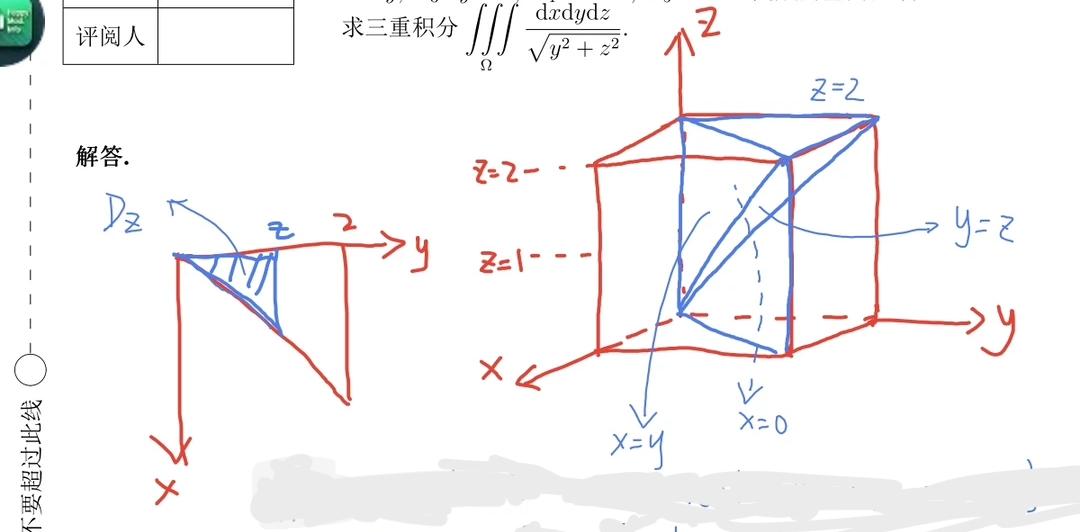
\includegraphics[width=0.6\textwidth]{cmc17.png}
\end{figure}




\begin{proof}
使用先二后一，对固定的 \(z\in[1,2]\)，有
\[
D_z=\{(x,y)\mid 0\le x\le y,\ 0\le y\le z\}.
\]
所以原积分
\begin{align*}
\iiint_{\Omega}\frac{\mathrm{d}x\,\mathrm{d}y\,\mathrm{d}z}{\sqrt{y^2+z^2}}
&=\int_1^2 \mathrm{d}z\int_0^z \mathrm{d}y\int_0^y
\frac{1}{\sqrt{y^2+z^2}}\,\mathrm{d}x\\
&=\int_1^2 \mathrm{d}z\int_0^z
\frac{y}{\sqrt{y^2+z^2}}\,\mathrm{d}y\\
&=\int_1^2 \sqrt{y^2+z^2}\Big|_0^z\,\mathrm{d}z\\
&=\int_1^2 \z(\sqrt{2}z-z\y)\,\mathrm{d}z\\
&=(\sqrt2-1)\int_1^2 z\,\mathrm{d}z\\
&=\frac{3}{2}(\sqrt2-1).
\end{align*}
\end{proof}

\end{document}
